% 1977 年辽宁卷第五题证法二：作 CE∥DB 交 AB 的延长线于 E，DBEC 为平行四边形
% （按源卷第 3 页「第五题证法二附图」布局；E 在 B 右侧，CE 与 DB 平行，BE 为延长线虚线）
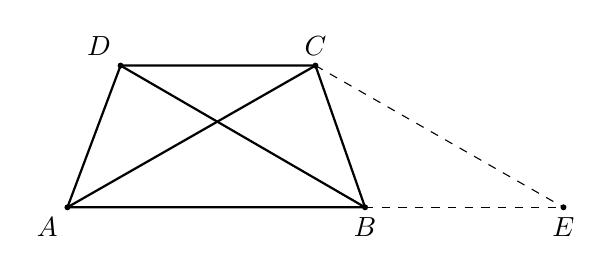
\begin{tikzpicture}[scale=0.9]
  \coordinate (A) at (0,0);
  \coordinate (B) at (4.2,0);
  \coordinate (D) at (0.75,2.0);
  \coordinate (C) at (3.5,2.0);
  \coordinate (E) at (7.0,0);
  \draw[thick] (A)--(B)--(C)--(D)--cycle;
  \draw[thick] (A)--(C);
  \draw[thick] (B)--(D);
  \draw[dashed] (C)--(E);
  \draw[dashed] (B)--(E);
  \fill (A) circle (1.2pt) node[below left] {$A$};
  \fill (B) circle (1.2pt) node[below] {$B$};
  \fill (D) circle (1.2pt) node[above left] {$D$};
  \fill (C) circle (1.2pt) node[above] {$C$};
  \fill (E) circle (1.2pt) node[below] {$E$};
\end{tikzpicture}
